%%%%%%%%%%% Single Column %%%%%%%%%%%%%%%%%
\documentclass[review, 1p, number, sort&compress,table]{elsarticle}
%%%%%%%%%% Double Column %%%%%%%%%%%%%%%%%%%
%\documentclass[preprint, 3p, twocolumn, number, sort&compress,table]{elsarticle}
%%%%%%%%%%%%%%%%%%%%%%%%%%%%%%%%%%%%%%%%%%%%%   
\journal{Acta Materialia}

\usepackage{styles/mainStyles}   % Set for for extra stylings
\usepackage{epstopdf}
% hyperlinking is set to color blue.
% \autoref is currently set to cross references figures as 'Fig. 1', and equations as 'Eq.1'. 
%This can be changed
%%%%%%%%%%%%%%%%%%%%%%%%%%%%%%%%%%%%%%%%%%%%
% --------------Custom Commands-------------%
%for more info go to ``styles\mainStyles.sty''
% \textgreek - enables greek letters outside of math mode (ie. \textalpha, \textgamma)
% \celcius   - for degrees C  
% \etal      - produces italic ``et al.''
% \um        - for micrometers
% \mc{23}{6}  - produces ``M23C6'' carbides. Can change values.
% Various Differential equation --- look at documentation for mor info 
%%%%%%%%%%%%%%%%%%%%%%%%%%%%%%%%%%%%%%%%%%%%
\begin{document}

	\begin{frontmatter}
	
		\title{title}
		
		\author[UoA]{X.~Y.~Jimmy\corref{cor1}}
			\ead{jimmy@ualberta.ca}

		
		\author[UoA]{P.~F.~Mendez}
			\ead{pmendez@ualberta.ca}
		
		\cortext[cor1]{Corresponding author. Tel: +1-780-XXX-XXXX}
		
		\address[UoA]{Department of Chemical and Materials Engineering, University of Alberta, Edmonton, Alberta,T6G 2V4, Canada}
	
		\begin{abstract}
			Abstract goes here
		\end{abstract}
		
		\begin{keyword}
			keyword1 \sep keyword2 \sep keyword3 \sep keyword4
		\end{keyword}

	\end{frontmatter}
	
	%%%%%%%%%%%%%%%%%%%%%%%%%%%%%%%%%%%%%%%%%%%%%%%%%%
%%%             INTRODUCTION SECTION              %%%%
%%%%%%%%%%%%%%%%%%%%%%%%%%%%%%%%%%%%%%%%%%%%%%%%%%	

	\section{Introduction}
		\indent introsection from  Mathes \etal, \cite{MOR91, texbook}, at 700 \celcius, and 300\um
		
		\small
		\begin{eqnarray}
		\label{eq:pfactor}
			\rm P&=&\rm{}7\times C + 5 \times Si - 3 \times Mn + 8 \times Nb \\ 
			  &:&\rm C,Si,Mn,Nb(wt\%)\nonumber
		\end{eqnarray}
		\normalsize
		
		 \autoref{eq:pfactor} in \cite{dB93}.           
		
	%%%%%%%%%%%%%%%%%%%%%%%%%%%%%%%%%%%%%%%%%%%%%%%%%%
%%%             EXPERIMENTAL SECTION              %%%%
  %%%%%%%%%%%%%%%%%%%%%%%%%%%%%%%%%%%%%%%%%%%%%%%%%%
  		
	\section{Experimental}\label{sec:experimental}
	  \subsection{Materials}
	  	Experimental section. \mc{23}{6}
			
	\begin{table*}[ht!]\scriptsize
		\renewcommand{\arraystretch}{1.2}
		\centering
		\caption{Composition of the ex-service 2032-Nb stainless steel alloy}
			\begin{tabular}{lccccccccc}
			\toprule%
					& \multicolumn{8}{c}{Composition (wt\%)}              \\\hline\noalign{\smallskip}
											     						& Cr    & Ni   & Mn   & Si   & C     & Nb   & N 		& W,Mo,Ti,Zr & $\rm{\frac{Nb}{(C+6/7N)}}$ Ratio \\\hline\noalign{\smallskip}
				 	2032Nb											& 20.6  &	32.7 & 0.96 & 1.00 & 0.086 & 1.13 & 0.051 & $<0.05$  	 & 8.71 \\ \bottomrule%
			\end{tabular}
			\label{tab:chemAnal}
	\end{table*}
	  	
		\subsection{Chemical analysis}
			\autoref{tab:chemAnal}
		
%%%%%%%%%%%%%%%%%%%%%%%%%%%%%%%%%%%%%%%%%%%%%%%%%%
%%%              RESULTS SECTION              %%%%
%%%%%%%%%%%%%%%%%%%%%%%%%%%%%%%%%%%%%%%%%%%%%%%%%%		    
  
\section{Results}\label{sec:results}
	\subsection{Model}
		The shear stress varies little within a thin shear layer, and will be assumed to have a
constant value $\tau_c$ in that region. Also, considering that the shear rate and velocity gradient are essentially the
same magnitude ($\dot\gamma=-\ltd{v}{x}$) we can restate as

\begin{equation}\label{eq:SL_heat_restated}
        q(x)=-\eta_s\tau_c\td vx
\end{equation}
with boundary condition $v=\omega a$ at $x=0$. The two terms of \autoref{eq:SL_heat_restated} can be normalized by
an estimation of their maximum values obtaining

\begin{equation}\label{eq:SL_heat_normalized}
            q_cq^*=-\frac 32\eta_s\tau_c\frac{\omega a}\delta\ntd vx
\end{equation}
where the magnitudes with an asterisk have been normalized by an estimation of their maximum value. The factor of 3/2
present in the normalization of the derivative relates to the  evolution of velocity within the shear layer illustrated in. Replacing the normalized functions by $+1$ or $-1$, \autoref{eq:SL_heat_normalized} turns into the following algebraic equation based on characteristic values:

\begin{equation}\label{eq:SL_heat_algebraic}
            \widehat{q_c}=\frac 32\eta_s\widehat{\tau_c}\frac{\omega
            a}{\widehat{\delta}}
\end{equation}

\autoref{eq:SL_heat_algebraic} introduces one new unknown characteristic value: $\widehat{\tau}$.

\ifpdf
	\begin{figure*}[ht!]
				\centering	
				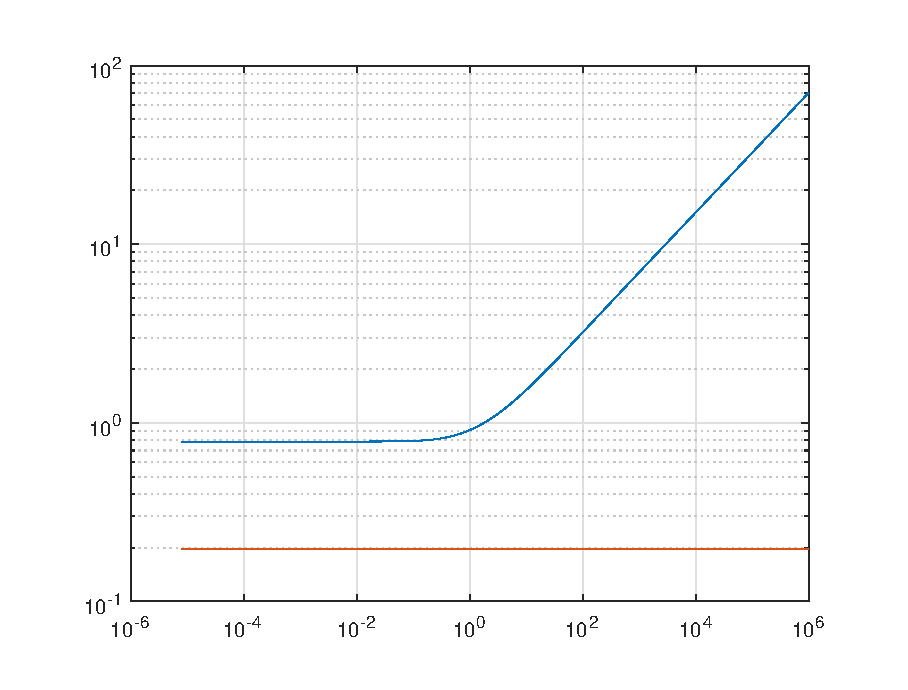
\includegraphics[width=6in]{1}
			\caption{Ratio of maximum temperature in the base plate $f_T$. The four hypotheses are fulfilled and the ratio
				remains relatively constant and close to unity.}	
			\label{fig:theta-pe}
	\end{figure*}
\else
		\begin{figure*}[!h]
		\centering
				\psfrag{theta=Ts/Ts}[c][c]{$f_T=\displaystyle \frac{T_s-T_{\infty}}{\widehat{T_s}-T_{\infty}}$}
				\psfrag{Pe}[c][c]{$\Pe$}
				\psfrag{Roy et al. Al6061 Num}[l][l][0.9]{\scriptsize Roy \etal Al6061 Num~\cite{roy06}}
				\psfrag{Roy et al. Al6061 Exp}[l][l][0.9]{\scriptsize Roy \etal Al6061 Exp~\cite{roy06}}
				\psfrag{Nandan et al. Al6061 Num}[l][l][0.9]{\scriptsize Nandan \etal Al6061 Num~\cite{nandan06mmta1247}}
				\psfrag{Nandan et al. Al6061 Exp}[l][l][0.9]{\scriptsize Nandan \etal Al6061 Exp~\cite{nandan06mmta1247}}
				\psfrag{Khandkar Al6061 Num}[l][l][0.9]{\scriptsize Khandkar \etal Al6061-T651 Num~\cite{khandkar03}}
				\psfrag{Khandkar Al6061 Exp}[l][l][0.9]{\scriptsize Khandkar \etal Al6061-T651 Exp~\cite{khandkar03}}
				\psfrag{Chen and Kovacevic Al6061-T6 Num}[l][l][0.9]{\scriptsize Chen and Kovacevic Al6061-T6 Num~\cite{chen03mtm1319}}
				\psfrag{Sato Al6063-T5 Exp}[l][l][0.9]{\scriptsize Sato \etal Al6063-T5 Exp~\cite{sato02}}
				\psfrag{Yang et al. Al2024-T351 Num}[l][l][0.9]{\scriptsize Yang \etal Al2024-T351 Exp~\cite{yang04}}
				\psfrag{Schmidt et al. Al2024-T3(2004) Exp}[l][l][0.9]{\scriptsize Schmidt \etal Al2024-T3 Exp~\cite{schmidt04msmse143}}
				\psfrag{Schmidt and Hattel Al2024-T3 Num(2005)}[l][l][0.9]{\scriptsize Schmidt and Hattel Al2024-T3 Num~\cite{schmidt05stwj177}}
				\psfrag{Schmidt and Hattel Al2024-T3 Exp(2005)}[l][l][0.9]{\scriptsize Schmidt and Hattel Al2024-T3 Exp~\cite{schmidt05msms77}}
				\psfrag{Colligan Al5083-H116 Exp}[l][l][0.9]{\scriptsize Colligan Al5083-H116 Exp~\cite{colligan07}}
				\psfrag{Reynolds et al. Al7050-T751 Num(2003)}[l][l][0.9]{\scriptsize Reynolds \etal Al7050-T751 Num~\cite{reynolds03msf2959}}
				\psfrag{Reynolds et al. Al7050-T7451 Num(2005)}[l][l][0.9]{\scriptsize Reynolds et al. Al7050-T7451 Num~\cite{reynolds05stwj190}}
				\psfrag{Roy et al. AISI 1018 Num}[l][l][0.9]{\scriptsize Roy \etal AISI 1018 Num~\cite{roy06}}
				\psfrag{Roy et al. AISI 1018 Exp}[l][l][0.9]{\scriptsize Roy \etal AISI 1018 Exp~\cite{roy06}}
				\psfrag{Nandan et al. AISI 1018 Num}[l][l][0.9]{\scriptsize Nandan \etal AISI 1018 Num~\cite{nandan06mmta1247}}
				\psfrag{Roy et al. AISI 304 Num}[l][l][0.9]{\scriptsize Roy \etal AISI 304 steel Num~\cite{roy06}}
				\psfrag{Correction function f(d/a)}[l][l][0.9]{\scriptsize Minimum squares trendline}
				\includegraphics[width=6in]{theta_pe}
				\caption{Ratio of maximum temperature in the base plate $f_T$. The four hypotheses are fulfilled and the ratio
				remains relatively constant and close to unity.}
				\label{fig:theta-pe}
		\end{figure*}
\fi

Near the incipient melting temperature, the Arrhenius component can be linearized as

\begin{equation}\label{eq:arrhenius_simplified}
	\exp\left(-\frac Q{R\widehat{T_s}}\right)\approx\left\{
	\begin{array}{cl}
	0&\mbox{if }T\leq T_0\\ \\\displaystyle{
	\frac{\widehat{T_s}-T_0}{T_m-T_0}\exp\left(-\frac{Q}{RT_m}\right)}&\mbox{if
	}T>T_0
	\end{array}
	\right.
\end{equation}

where $T_m$ is the temperature of incipient melting of the material, whether its solidus temperature or some critical
low melting temperature eutectic.

\subsection{Chemistries}
	
	\begin{table*}[ht!]\tiny
			\centering
			%\renewcommand{\arraystretch}{2}
			\caption{Phase composition in wt\%(brackets in at\%) on the microstructure of a fully aged centrifugally cast 20Cr-32Ni-1Nb stainless steel sample. Compositional data was gathered using AES quantitative Analysis.}

				\begin{tabular}{p{1.7cm}lllllllp{1cm}}
					\toprule%
								& \multicolumn{7}{c}{Composition, wt\%(at\%)} &  \\\hline\noalign{\smallskip}
					Phase 						& Fe 	& Ni 																									 & Cr 																									 & Si  																								    		& Nb 																			 							& C 																											& N 																							 			 	& Number of Points \\\hline\noalign{\smallskip}
					  Fully Aged  &&&&&&&& \\
					  \hline\\
					\\
	\parbox[t]{1.6cm}{$\gamma$-Fe \\(boundary)} & bal &\parbox[t]{1.6cm}{36.7 $\pm$ 1.6 \\ (32.3 $\pm$ 2.0)} 	&\parbox[t]{1.6cm}{17.50 $\pm$ 3.8 \\ (17.3 $\pm$ 3.2)}   & -   																								       & -  																		 							& \parbox[t]{1.6cm}{2.43 $\pm$ 1.4\\ (10.2 $\pm$ 5.6)}  		& - 																							 	& 4   \\[7mm]
					Z-Phase 					& bal	& \parbox[t]{1.6cm}{1.4 $\pm$ 1.6 \\ (1.2 $\pm$ 1.4)} 	& \parbox[t]{1.6cm}{31.1 $\pm$ 1.2 \\ (29.2 $\pm$ 0.7)}  & \parbox[t]{1.6cm}{0.2 $\pm$ 0.6 \\ (0.4 $\pm$ 1.0)} & \parbox[t]{1.6cm}{55.4 $\pm$ 2.0 \\ (29.1 $\pm$ 1.7)} & \parbox[t]{1.6cm}{1.4 $\pm$ 0.3 \\ (5.6 $\pm$ 1.0)} & \parbox[t]{1.6cm}{9.7 $\pm$ 0.8 \\ (33.9 $\pm$ 2.0)}   			& 14 \\[7mm]
					$\rm M_{23}C_{6}$ & bal & \parbox[t]{1.6cm}{3.3 $\pm$ 0.6 \\ (2.5 $\pm$ 0.5)} 	& \parbox[t]{1.6cm}{82.7 $\pm$ 0.7 \\ (70.9 $\pm$ 1.7)} &  -
				& -																									 	& \parbox[t]{1.6cm}{5.3 $\pm$ 0.6 \\ (19.6 $\pm$ 2.0)} 		& - 																								& 12 \\[7mm]
					G-Phase 					& bal & \parbox[t]{1.6cm}{52.0 $\pm$ 3.4 \\ (48.6 $\pm$ 2.9)} & \parbox[t]{1.6cm}{0.3 $\pm$ 0.6 \\ (0.3 $\pm$ 0.6)} 		& \parbox[t]{1.6cm}{11.6 $\pm$ 1.5 \\ (22.5 $\pm$ 2.5)}& \parbox[t]{1.6cm}{33.6 $\pm$ 4.3 \\ (20.0 $\pm$ 3.0)} & \parbox[t]{1.6cm}{1.1 $\pm$ 0.2 \\ (5.2 $\pm$ 0.9)} 			& \parbox[t]{1.6cm}{0.7 $\pm$ 0.6 \\ (2.8 $\pm$ 2.4)} 	 & 14  \\[7mm]
					Nb(C,N) 					& bal & \parbox[t]{1.6cm}{7.3 $\pm$ 4.6 \\ (5.1 $\pm$ 3.0)} & \parbox[t]{1.6cm}{3.1 $\pm$ 4.0 \\ (2.6 $\pm$ 3.5)} 		& \parbox[t]{1.6cm}{1.0 $\pm$ 0.4 \\ (1.1 $\pm$ 0.3)}& \parbox[t]{1.6cm}{69.2 $\pm$ 5.8 \\ (31.1 $\pm$ 3.4)} & \parbox[t]{1.6cm}{12.2 $\pm$ 1.7 \\ (42.2 $\pm$ 4.0)} 			& \parbox[t]{1.6cm}{5.5 $\pm$ 0.7 \\ (16.4 $\pm$ 2.0)} 	 & 14  \\
					\\\hline
					  Annealed  &&&&&&&& \\
					\hline\\
					Nb(C,N) 					& bal & \parbox[t]{1.6cm}{4.8 $\pm$ 2.1 \\ (4.1 $\pm$ 2.5)} & \parbox[t]{1.6cm}{1.9 $\pm$ 1.7 \\ (1.8 $\pm$ 1.7)} 		& \parbox[t]{1.6cm}{1.1 $\pm$ 1.2 \\ (1.9 $\pm$ 2.1)}& \parbox[t]{1.6cm}{74.2 $\pm$ 5.8 \\ (39.2 $\pm$ 3.0)} & \parbox[t]{1.6cm}{8.9 $\pm$ 0.7 \\ (36.5 $\pm$ 2.4)} 			& \parbox[t]{1.6cm}{3.3 $\pm$ 0.4 \\ (11.4 $\pm$ 1.4)} 	 & 25  \\\bottomrule
				\end{tabular}
			\label{tab:AESAged}
		\end{table*}
			
\indent The results in \autoref{tab:AESAged}   
	
	\begin{table}[ht!]\scriptsize
		\renewcommand{\arraystretch}{1.2}
		\caption{Particle diameter, and phase fraction (vol\%) of a fully aged, and solution annealed 2032Nb microstructure.}
		\begin{center}
			\begin{tabular}{l|cp{1cm}c}
			%\begin{tabular}{l|>{\columncolor[gray]{.8}}c>{\columncolor[gray]{.8}}p{1cm}>{\columncolor[gray]{.8}}c|cp{1cm}c}
			\toprule%
															&   \multicolumn{3}{c}{Centrifugally Cast} \\\hline\noalign{}%{\smallskip}

					Phase 							& \parbox[t]{1.8cm}{particle \\Diameter \\ ($\mu{}m$)} & Number of Points & \parbox[t]{1.6cm}{Phase  \\ Fraction \\(vol\%)} \\
					\hline%\noalign{}{\smallskip}
					\multicolumn{2}{l}{Fully Aged} & & \\ 
					\hline
				 	Nb(C,N) 						& 1.73 $\pm$ 1.17 		 & 14		& 0.03 $\pm$ 0.01 \\
				 	$\rm{M_{23}C_{6}}$ 	& 2.86 $\pm$ 1.52 		 & 85 	&	0.97 $\pm$ 0.32 \\
				 	\parbox[t]{1.8cm}{G-phase \\
				 	(interdendritic)}		& 4.02 $\pm$ 2.00			 & 68 	& 2.43 $\pm$ 0.48 \\
				 	\parbox[t]{1.8cm}{G-phase \\
				 	(intradendritic)}		& 1.33 $\pm$ 0.30			 & 108	& 0.92 $\pm$ 0.12 \\
				 	Z-phase 						& 1.50 $\pm$ 0.83 		 & 49		& 0.29 $\pm$ 0.16 \\
				 	\hline
					 \multicolumn{2}{l}{Solution Annealed} & &\\
				 	\hline
				 	Nb(C,N)             & 0.78 $\pm$ 0.23			 & 129  & 3.40 $\pm$ 0.10 \\
				 \bottomrule%
			\end{tabular}
			\end{center}
			\label{tab:AgedSizeFraction}
	\end{table}
	\indent \autoref{tab:AgedSizeFraction} includes the area fraction, and precipitate diameter for each phase characterized in AES, and SEM. For every phase except Z-phase, Area fractions were obtained by EPMA elemental mapping on the center of each sample. The resolution of the elemental maps was 1\um/pixel, at a dwell time of 20ms, where the area fractions were calculated from a total area of $531mm^{2}$.
	
% For a 347 stainless steel alloy Z-phase becomes a stable phase with alloy additions greater than 0.06 wt\% nitrogen.
	\subsection{Phase Mapping}
	
	\begin{figure*}[ht!]
		\begin{center}$
			\begin{array}{cc}
				\includegraphics[width=3in]{AES_Map/BSE} & \includegraphics[width=3in]{AES_Map/Nb} \\
				\includegraphics[width=3in]{AES_Map/C} & \includegraphics[width=3in]{AES_Map/N} \\
				\includegraphics[width=3in]{AES_Map/Cr} & \includegraphics[width=3in]{AES_Map/Si} \\
			\end{array}$
		\end{center}
		\caption{Element maps from Auger Electron Spectroscopy of an interdendritic region of a fully aged 2032Nb Stainless steel pipe.}
		\label{fig:aesmap}
	\end{figure*}

\subsection{ThermoCalc \&  Compositional Factorial Design}

	\begin{figure}[H]
		\begin{center}
			\includegraphics[width=3in]{phase}	
		\end{center}			
		\caption{Equilibrium phase fraction in mol \% predicted by ThermoCalc using the TCFE6, and TTNI8 databases for the centrifugally cast 2032-Nb stainless steel chemistry in \autoref{tab:chemAnal}.}	
			\label{fig:thermoPhase}
	\end{figure}
	
	\indent Say some stuff about \autoref{fig:thermoPhase}. Now here is a figure with subfigures inside of it.
	
\captionsetup[subfigure]{position=top}
\begin{figure*}[ht!]
	\begin{center}
		\subfloat[]{\label{fig:hara2008-Fig1}\includegraphics[width=2.2in]{hara2008-Fig1}}
		\subfloat[]{\label{fig:hara2008-Fig2}\includegraphics[width=2.2in]{hara2008-Fig2}}
		\subfloat[]{\label{fig:hara2008-Fig3}\includegraphics[width=2.2in]{hara2008-Fig3}}
	\end{center}
	\caption{Relationship between the change in cooling rate with the (a) 50\% $\gamma/\alpha$ transformation temperature, (b) hardness, (c) $\gamma/\alpha$ start transformation temperature.}
	\label{fig:hara2008-coolingRate}
\end{figure*}
	
%%%%%%%%%%%%%%%%%%%%%%%%%%%%%%%%%%%%%%%%%%%%%%%%%%
%%%              DISCUSSION SECTION              %%%%
%%%%%%%%%%%%%%%%%%%%%%%%%%%%%%%%%%%%%%%%%%%%%%%%%%		      
\section{Discussion}\label{sec:discussion}

\subsection{Revised Objective Function}
	 Since the actual value of the objective function is not important for this model, variables y(p,i,j) and z(p,i,j) can be optimized for each player by adding their cost products to the objective function.
	
\begin{equation} \label{eq:obj}
	  \rm max\; z\: := \: \sum_{p \in P}\sum_{i \in N}\sum_{j \in M}{c(i,j)x(p,i,j)}
	\end{equation} 
	
	First of all, the resource matrix is converted into binary arrays for each of the five resources. for example:
	\[ \rm
	 lbr(i,j) = \left\{ \begin{array}{ll} 
									\rm 0\; ,\; if\: res(i,j) > 1\\
									\rm 1\; , \; if\: res(i,j) = 1 \\
								 \end{array}\right.
	\]
	For multiple equations
	\begin{align*} \label{eq:cityW}
			\rm \sum_{i \in N}\sum_{j \in M}{l(i,j)z(p,i,j)} \leq 3(1-\delta(p)) \; &\forall \; p \in \{1 \ldots 4\} \\
			\rm \sum_{i \in N}\sum_{j \in M}{b(i,j)z(p,i,j)} \leq 3(1-\delta(p)) \; &\forall \; p \in \{1 \ldots 4\} \\
			\rm {x(p,i,j) - w(i,j)} \leq 3(\delta(9-p)) \; &\forall \; \{p \in \{4 \ldots 8\}, i \in N, j \in M \}
	\end{align*}	


	 
%\begin{itemize}
%	\item nitrogen can be used to limit the amount of G-phase, but not eliminate it all together. This may not alleviate the liquation cracking problems. There is also the question of what Z-phase and potentially $\pi$-phase would do to the alloy, negative or positive. Can only relate to microstructure analyzed by Danielson for clues.
%	\item carbon influence on $\rm M_{23}C_{6}$
%	\item $\pi$-phase precipitates at the expense of Z-phase. Increased Si will promote $\pi$-phase. Nb promotes Z-phase or G-phase at expense of $\pi$-phase.
%	\item high carbon and nitrogen content forces high stability temperature for $\rm M_{23}C_{6}$ because of Nb/(C+N) ratio.
%\end{itemize}
	      
%%%%%%%%%%%%%%%%%%%%%%%%%%%%%%%%%%%%%%%%%%%%%%%%%%
%%%              CONCLUSIONS SECTION              %%%%
%%%%%%%%%%%%%%%%%%%%%%%%%%%%%%%%%%%%%%%%%%%%%%%%%%		

	\section{Conclusions}
	\indent Conclusions Section

%%%%%%%%%%%%%%%%%%%%%%%%%%%%%%%%%%%%%%%%%%%%%%%%%%
%%%              Acknowledgement SECTION              %%%%
%%%%%%%%%%%%%%%%%%%%%%%%%%%%%%%%%%%%%%%%%%%%%%%%%%	
	\section{Acknowledgement}
	\indent This study has been supported by...      			
	
\section{References}
\bibliography{References/references}   % .bib info
%%%%%%%%%%%%%%%%% Reference Style %%%%%%%%%%%%%%%%%%%
% Needs to be changed based on the journal you are sumbitting to. 
% see ``bst\journal_refstyles.pdf'' for more information
\bibliographystyle{bst/model3-num-names}		

\end{document}